\documentclass{cmc}
\usepackage{makecell}
\usepackage{enumitem}
\usepackage{amsmath}

% \usepackage{subfig}
\begin{document}

\pagestyle{fancy}
\lhead{\textit{\textbf{Computational Motor Control, Spring 2024} \\
    Final project, Project 1, GRADED}} \rhead{Student \\ Names}

\section*{Student names: \ldots (please update)}

\textit{
  Please note that this project is \textbf{\corr{graded}}. \textbf{\corr{The project will be graded in two parts}}.
  \begin{itemize}
  \item In Part 1(Project 1) you will implement and analyze a wave controller to actuate a zebrafish model to study
  swimming in water.
  \item Part 2(Project 2) is divided in two subparts:
  \begin{itemize}
  \item In the first part you will implement and analyze a biophysically inspired neural network firing rate controller.
  \item In the second part you will incorporate stretch feedback neurons in the the firing rate controller and study the role of stretch during swimming.
  \end{itemize}
  \end{itemize}
  The two projects' submissions will be done separately. The code useful to complete the project will be updated on the repository under the folder Project/ (if necessary) after each project part assigment.
  This file is the Assignment for Project 1.
}

\textit{
  \textbf{\corr{Deadlines: Project 1: Friday 26/04/2024 23:59, Project 2: Friday 07/06/2024 23:59, }}
}

\textbf{Instructions}

\begin{itemize}
  \item \textit{
    Update this file (or recreate a similar one, e.g.\ in
    Word) to prepare your answers to the questions. Feel free to add text,
    equations and figures as needed. Hand-written notes, e.g.\ for the development
    of equations, can also be included e.g.\ as pictures (from your cell phone or
    from a scanner). The code of project 1 should contain exercise 1a to 1c.
  }
  \item \textit{ Please submit both the source file.
    (*.doc/*.tex) and a pdf of your document, as well as all the used and updated
    python code can be submitted in a single zipped file called \newline
    \corr{final\_report\_name1\_name2\_name3.zip} where name\# are the team
    member's last names.  \corr{Please submit only one report per team!}
  }
\end{itemize}

%%%%%%%%%%%%%%%%%%%%%%%%%%%%%%%%%%%%%%%%%%%%%%%%%%%%%%%%%%%%%%%%%%%%%%%%%%%%%%%%%%%%%%%%%%%%%%%%%%%%
% \section*{Questions}
\section*{Project overview and motivations - the zebrafish as a case of study}\label{sec:exploring-swimming}

The zebrafish (Fig \ref{fig:zebrafish}) is a key animal model in biology and neuroscience.

\begin{figure}[H]
  \centering
  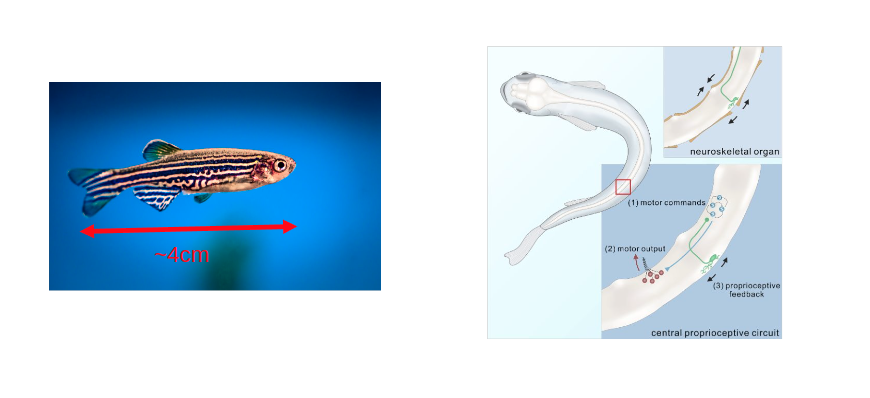
\includegraphics[width=1\textwidth]{figures/zebrafish.png}
  \caption[zebrafish]{The zebrafish}\label{fig:zebrafish}
\end{figure}

In Project 1 and 2 you will model and simulate swimming in an adult zebrafish. It is known
that zebrafish can generate swimming at three regimes (slow, medium and fast swimming). Here
you will implement a controller for generating slow swimming (1-4Hz).

Interestingly, it was recently found that these animals are equipped with proprioceptive sensitive organs
that sense the local stretch and use it to sense the environmental changes and update its swimming
behavior, but its role is still unclear. This will be the topic of the next part of the project(Project 2).

In these projects you will have the opportunity to explore this puzzling experimental findings by
building and testing a full model of the zebrafish locomotion. You will use Python and the MuJoCo physics
engine to control a neuromechanical model of the zebrafish, and test some hypothesis of the working principles
of the locomotion of these animals.



\subsection*{Simulation environment installation}

Before digging into the details of the project, let's first install all the tools
needed to run the simulations and test the interactive GUI of the simulation environment.


\section*{Prerequisites}
To have all the necessary python packages necessary to complete the
final project, check that you have installed all the necessary required packages.

\corr{\textit{IMPORTANT:}} Make sure you have activated and are using your
virtual environment and its python interpreter that that you have created for
this course.

\corr{\textit{NOTE:}} If you are unclear about the basic steps then refer back
to Lab 0 documentation

Next, pull the latest version of the exercise repository. Navigate to the
directory \textit{Project1/Python} in the terminal and execute the following,

\begin{lstlisting}[language=Bash]
  >> pip install -r requirements.txt --upgrade
\end{lstlisting}

Next, download the zip folder \textit{farms\_packages.zip} uploaded in Moodle and unzip its content
in a desired directory. Copy in this directory the python file \textit{setup\_sim\_env.py}.
and run inside the zipped directory it by simply calling:

\label{sec:mujoco-inst}
\begin{lstlisting}[language=Bash]
  >> python setup_sim_env.py
\end{lstlisting}

This will install the \textit{MuJoCo} simulator and the \textit{dm\_control}
package which are software maintained by Deepmind for running multi-body rigid system
simulations. It will also install the \textit{farms\_core},
\textit{farms\_mujoco}, \textit{farms\_amphibious} and \textit{farms\_sim} FARMS packages developed at the
Biorobotics Laboratory (BioRob). If you are interested in knowing more about
\textit{MuJoCo} and FARMS, you can find out more on \href{https://mujoco.org/}{\corr{the
    official website}} and \href{https://www.biorxiv.org/content/10.1101/2023.09.25.559130v1https://www.biorxiv.org/content/10.1101/2023.09.25.559130v1}{\corr{the FARMS paper}}



\subsection*{Examples}
You can run a simulation example to get you accustomed
to the MuJoCo graphical interface with \corr{\textbf{example\_single.py}}. You
should see the polymander model floating on the water. Try running:
\label{sec:first-example}
\begin{lstlisting}[language=Bash]
  >> python example_single.py
\end{lstlisting}

\subsubsection*{Graphical User Interface Interaction}
When you run the example script, a Graphical User Interface (GUI) should launch.
You can use the left mouse click to move around the scene and right mouse click
to rotate the camera. You can also select a part of the robot by double left
clicking on a part. Once selected, you can then interact with it by holding the
CONTROL key and dragging with left or right click. Try it out for yourself to
familiarise with the interface.

There are many keyboard shortcuts also available

\begin{itemize}
\item Press SPACE to toggle play/pause
\item Press ``\textquotesingle'' / ``\textsuperscript{$\wedge$}'' to change
  speed factor (between zero (0) and backspace)
\item Press w to toggle wireframe
\item Press t to toggle transparency
\item Press s to toggle shadows
\item Press c to show collisions
\item Press f to show collisions forces, combine with p to show
  friction/reaction
\item Press b to show external forces (try in water later on)
\item And many more...
\end{itemize}


\section*{The mechanical model}\label{sec:mechanical}
The mechanical zebrafish model consists of $n_{links}=16$ links connected by $n_{joints}=15$
rotational yaw torques as in \ref{fig:mechanical} that are modeled using an
Ekeberg spring-mass-damper muscle model.

\begin{figure}[ht]
  \centering 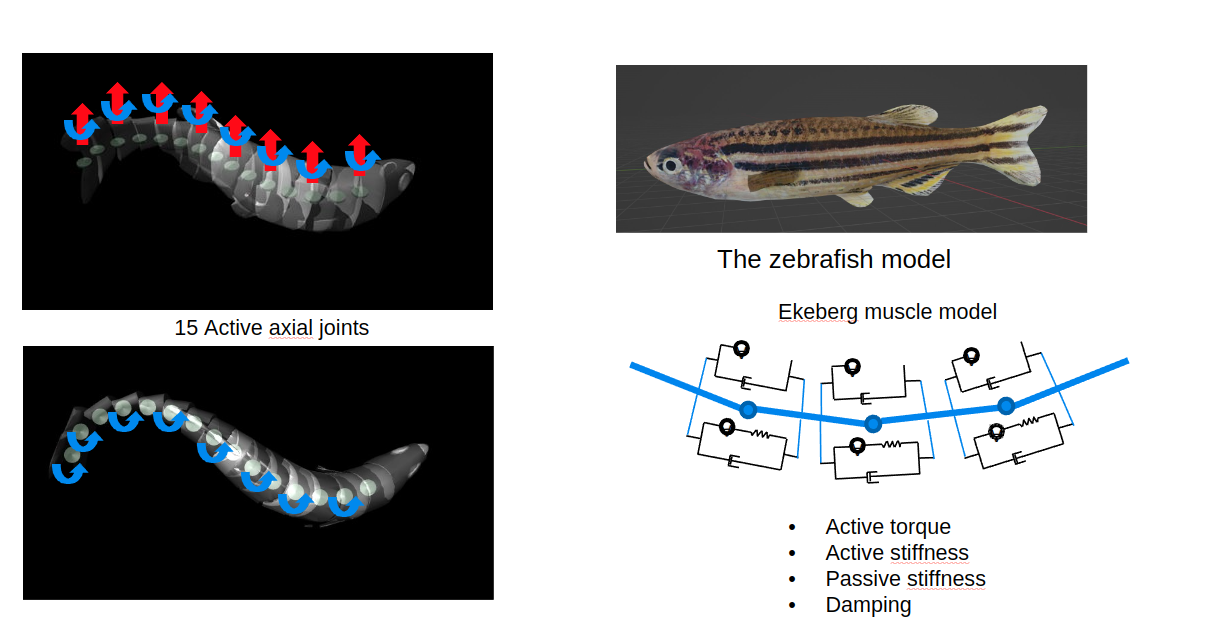
\includegraphics[width=1.0\textwidth]{figures/mechanical.png}
  \caption{\label{fig:mechanical} The mechanical model of the zebrafish}
\end{figure}


\begin{figure}[ht]
  \centering 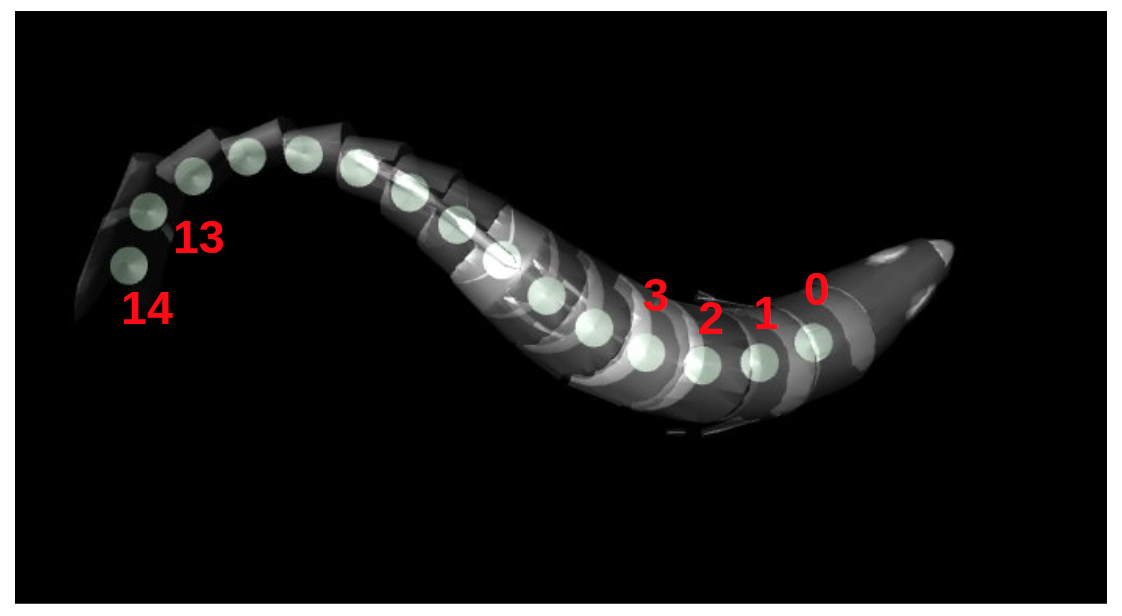
\includegraphics[width=1.0\textwidth]{figures/joints.png}
  \caption{\label{fig:mechanical2} The joint numbering}
\end{figure}

The activity of muscle cells on each joint is transduced in output torques for
the mechanical model by means of Ekeberg Muscle Models (\ref{fig:mechanical}).

For each joint $i=0,...,14$, the model receives in input the left ($M_{L_i}$) and right ($M_{R_i}$)
activations from the muscle cells, and the current joint angle ($\theta_i$) and speed ($\Dot{\theta_i}$)
to compute the resulting output torque ($\tau_i$) via:

\begin{eqnarray}
\label{eq:electro_mechanical}
	\tau_i = \alpha_i M_{diff_i} + \beta_i(\gamma_i +M_{sum_i} )\theta_i + \delta_i \Dot{\theta_i} \\
    M_{diff_i} = (M_{L_i} - M_{R_i}) \\
    M_{sum_i} = (M_{L_i} + M_{R_i})
\end{eqnarray}
Where $\alpha_i$ is the active gain, $\gamma_i$ is the passive stiffness, $\beta_i$ is the active stiffness, $\delta_i$ is the damping coefficient. The Ekeberg muscle model is a rotational spring-damper system with the addition of a variable stiffness term $\beta (M_L+M_R) \theta_i$. The active term of the model acts an external torque $\alpha(M_L-M_R)$.

The Ekeberg model parameters have already been optimized (you do not need to change them).

The water is simulated using a simplified drag model.

% \newpage

\subsection*{Code organization}\label{subsec:code}

In this exercise you will modify the files \fileref{exercise\_\#.py}, \fileref{wave\_controller.py}, \fileref{simulation\_parameters.py} (optional) and \fileref{plot\_results.py} (optional). We provide below
a brief description of these and the other files, for completeness.

\begin{itemize}
\item \corr{\textbf{example\_single.py}} --- Run single simulation example (fixed parameters)
\item \corr{\textbf{example\_multiple.py}} --- Run multiple parallel simulations with different parameters
\item \corr{\textbf{exercise\_\#.py}} --- Files for the exercises 1-3
\item \corr{\textbf{wave\_controller.py}} --- This file contains the equations for the left and right muscle activations in a step function, which is internall called at each iteration time step. It also contains the metrics dictionary.
\item \corr{\textbf{simulation\_parameters.py}} --- This file contains the
  SimulationParameters class and is provided for convenience to send parameters
  to the setup of the controller. Please carefully read the parameter list
  and their documentation in this code.
\item \corr{\textbf{metrics.py}} --- This file contains the implementation
  for all the controller/mechanical metrics (see below).
\item \corr{\textbf{plotting\_common.py}} --- Plotting utilities (see below).
\item \corr{\textbf{plot\_results.py}} --- Loading and plotting the simulation results.
\item \corr{\textbf{util folder}} --- Contains all the utilities for running the simulation (do not modify)	
\item \corr{\textbf{logs folder}} --- Contains all the simulation logs
\item \corr{\textbf{muscle\_parameters folder}} --- Contains the optimized muscle parameters used in the Project (do not modify)
\item \corr{\textbf{models folder}} --- Contains extra code for the biomechanical and simulation in MuJoCo (do not modify)
\end{itemize}


\subsection*{Evaluating the performance}
In \corr{\textbf{util.metrics.py}}, we provide some basic functions to evaluate the performance
of the model simulations, and stored in the dictionary \corr{wave\_controller.py::WaveController.metrics} if the parameter compute\_metrics is greater than 0 (check \corr{simulation\_parameters.py}). These metrics are provided to you (you can use them to answer the question, or implement your own). Below we list the metrics and provide a brief description of how these are computed. All metrics are computed after discarting a $sim_fraction$ percentage of transient time point (currently $sim_fraction$ is set to 0.3, i.e. $30\%$ of the total simulation time but you can modify this if needed in \corr{\textbf{util.metrics.py}}). This is the assumed steady state fraction of time points. We distinguish between two different performance metrics:

\begin{enumerate}
\item \textbf{Controller metrics:} these are metrics related to the controller muscle activation signals $\overrightarrow{M}_{diff}=(M_{diff_i}=M_{L_i} - M_{R_i})_{i=1,...,N_{joints}}$, and assumes that the left and right signals $M_{L_i}$ and $M_{R_i}$ are stored in \fileref{wave\_controller.py::WaveController().state[:,self.muscle\_l]} and \fileref{wave\_controller.py\-::WaveController().state[:,self.muscle\_r]}, respectively, and converged to a steady state solution. We provide the following metrics:
	\begin{itemize}
	\item \textbf{frequency} - Stored in metrics["frequency"] (value $\in \mathbb{R}$). Computes the average frequency of the vector $\overrightarrow{M}_{diff}$ over the $N_{joints}$ joints from the time difference between zero threshold crossings (threshold crossing method) of each $M_{diff_i}$.
	\item \textbf{ptcc} - Stored in metrics["ptcc"] (value $\in [0,2]$). It's the peak-to-through correlation coefficients based on the difference between the the maximum and the minimum of the auto-correlogram of oscillatory signals. It measures the stability of the signals (value $\sim 2$=stable oscillations, value $<1.5$=unstable oscillations). 	
	\item \textbf{ipls} - Stored in metrics["ipls"]. Compute the sum time difference between zero threshold crossings of adjacent muscle $M_{diff_i}$ and $M_{diff_{i+1}}$
	\item \textbf{wavefrequency} - Stored in metrics["wavefrequency"] (value $\in \mathbb{R}$). Computes the wavefrequency of the muscle difference signals, i.e. metrics["frequency"]*metrics["ipls"].
		\item \textbf{amplitude} - Stored in metrics["amp"] (value $\in \mathbb{R}$), computes $\max(\overrightarrow{M}_{diff})-\min(\overrightarrow{M}_{diff})$.
	\end{itemize}
\item \textbf{Mechanical metrics:} these are metrics related to the mechanical model. We provide the following metrics:
	\begin{itemize}
	\item \textbf{Speed metrics}. We provide two different forward ($\vec{v}_{fwd} \in \mathbb{R}$) and lateral ($\vec{v}_{lat} \in \mathbb{R}$) speed metrics.
	\begin{enumerate}
	\item \textbf{PCA forward and lateral speeds}. Stored in metrics["fspeed\_PCA"] and metrics["lspeed\_PCA"] (values $\in \mathbb{R}$), respectively. \newline
	\textit{Advantage}: compute the instantaneous speeds \newline
	\textit{Disadvantage}: assumes that the body maintains an elongated position at all times (can produce large errors for large body bendings) \newline
	\textit{Explanations}: it computes the instantaneous speed of the center of mass ($\vec{v}_{com}(t)$) along the first ($\vec{PC}_1(t)$) and second ($\vec{PC}_2(t)$) principal components of the axial joints' coordinates $X(t)=(x(t),y(t))$ in the x-y dimensions, respectively. These coordinates are called $x_{axial}$ hereafter (total of $N_{njoints}=15$ axial joints). The projections are computed at each time step and integrated over the simulation to obtain their average values.
	\begin{equation}
	  \label{eq:pca1}
	    \vec{PC}_1(t) = argmax_{||a||=1}(\boldsymbol{a}^T Cov(\boldsymbol{X}(t)) \boldsymbol{a})
	\end{equation}

\begin{equation}
  \label{eq:pca2}
  \vec{PC}_2(t) = \vec{PC}_1(t) \times \hat{k}
\end{equation}

\begin{equation}
  \label{eq:xcom}
  \vec{x}_{com}(t) = \frac{1}{N_{joints}} \sum_{axial} \vec{x}_{axial}(t)
\end{equation}


\begin{equation}
  \label{eq:vcom}
  \vec{v}_{com}(t) = \frac{1}{dt} (\vec{x}_{com}(t) - \vec{x}_{com}(t-dt))
\end{equation}

\begin{equation}
  \label{eq:vfwd}
  \vec{v}_{fwd} = \frac{1}{T} \sum_t < \vec{v}_{com}(t), \vec{PC}_1(t) > dt
\end{equation}

\begin{equation}
  \label{eq:vlat}
  \vec{v}_{lat} = \frac{1}{T} \sum_t < \vec{v}_{com}(t), \vec{PC}_2(t) > dt
\end{equation}

This methods allows to maintain a notion of positive and negative speed as well as to measure
the curvature of the trajectory, two aspects that you will explore during the project.

	\item \textbf{Cycle forward and lateral speeds}. Stored in metrics["fspeed\_cycle"] and metrics["lspeed\_cycle"], respectively (values $\in \mathbb{R}$). \newline
	\textit{Advantage}: does not suffer for large body bendings computations \newline
	\textit{Disadvantage}: compute the speed computed across subsequent cycles (not instantaneous) and assumes oscillatory signals at steady state \newline
	\textit{Explanations}: Firstly, the algorithm computes the average frequency $f$ of the muscle difference signals $M_{diff_i}$ using the treshold crossing detection method (see controller metrics above). If $f>0$ (otherwise, the velocities are both zeros) it samples the joints coordinates across cycles and computes the velocity of the displacements of the head coordinates $X_{head}(t)=(x(t),y(t))$ between an initial time instant and a cycle of frequency $f$ before:
	
	\begin{equation}
  		\label{eq:vel_cycle}
  		v(t) = \frac{|X_{head}(t)-X_{head}(t-T)|}{T}
	\end{equation}
	Where $T=1/f \cdot dt$ is the period.
	The head to tail direction versor $\overrightarrow{ht}$ is then computed from the average angle between the first (head) and the second (neck) links across the considered cycle $\bar{\theta}$ as:
	\begin{equation}
  		\label{eq:theta}
  		ht= (\cos(\bar{\theta}),\sin(\bar{\theta}))
	\end{equation}
	The left pointing versor $\overrightarrow{ht}_{left}$ with respect to the $\overrightarrow{ht}$ direction is then computed using the right-hand rule.
	
	Finally, the forward and lateral speeds are respectively computed as the projection of the velocity $v$ along $\overrightarrow{ht}$ and $\overrightarrow{ht_{left}}$.
	
	\end{enumerate}
	\item \textbf{Torque consumption}. Stored in metrics["torque"] (value $\in \mathbb{R}$) and computes the total exerted torques as computed as the integral over time of the sum of all the torques (in absolute values)
generated by the joints.

\begin{equation}
  \label{eq:torques}
  T_{tot} = \sum_t \sum_{seg} || \tau_{seg}(t) ||
\end{equation}
	\end{itemize}
\end{enumerate}

Note that these metrics are to be intended as a reference for the generation of some of the plots but you
may implement new metrics that you think could be useful (i.e cost of transport).


\subsection*{Running the simulations}\label{subsec:simulating}
We provided two example files for running the simulations:
\begin{itemize}
\item \fileref{example\_single.py} - in this example you can see how to run a single simulation of the zebrafish (already tries in section \ref{sec:first-example}). You will explore the GUI, where to store the simulation data (for postprocessing and plotting) and how to use some plotting tools (explained more in the next section). Try to change some parameters of the \fileref{siumulation\_parameters.py} files to test how it works (try, i.e. to save the video, activate/deactivate the headless mode, etc).
\item \fileref{example\_multiple.py} - in this example you can see how to run multiple simulation (without GUI) in parallel using the processors for different parameter values.
\end{itemize}


\subsection*{Plotting tools (optional)}\label{subsec:plotting}
We provided some optional plotting tools in \fileref{plotting\_common.py} (check the documentation for more details):
\begin{itemize}
\item \fileref{plot\_time\_histories} - plots time histories of a vector of states on a single plot
\item \fileref{plot\_time\_histories\_multiple\_windows} - plots time histories of a vector of states on multiple subplots
\item \fileref{plot\_left\_right} - plotting left and right time histories on separate subplots
\item \fileref{plot\_2d} - plots an array 2d colored plot (uuseful for 2d parameter searches)
\item \fileref{plot\_trajectory} - plots head positions
\item \fileref{plot\_positions} - plots positions of the links

Examples for how to use these tools can be found in \fileref{example\_single.py} and \fileref{plot\_results.py}

\end{itemize}


% \newpage


\subsection*{Final notes}
\begin{itemize}
\item Use the exercise files \fileref{exercise\_X.py}, with X the exercise number to answer the question X, for example, \fileref{exercise\_0.py} to answer question 0.
\item Check the notes on the code. Many explanations are given therein.
\item Be concise and precise in the answers in the answers of the exercises.
\item You can append videos to explain your reasoning.
\end{itemize}



%%%%%%%%%%%%%%%%%%%%%%%%%%%%%%%%%%%%%%%%%%%%%%%%%%%%%%%%%%%%%%%%%%%%%%%%%%%%%%%%%%%%%%%%%%%%%%%%%%%
\newpage
\section*{Questions}
At this point you can now start to work on implementing your exercises.

\subsection*{1. Implement the equations for a sine wave controller}\label{sec:ex0}
Implement a sine wave swimming controller that generates a periodic traveling wave for the left and right muscle activations ($M_{L_i}$ and $M_{R_i}$, for $i=0,...14$) to actuate the zebrafish according to equation \ref{eq:sine_controller}.

\begin{eqnarray}
  \label{eq:sine_controller}
M_{L_i} (t)&=0.5 + \frac{A}{2} \cdot \sin \left( 2 \pi f \cdot \left( t - \epsilon \cdot \frac{i}{N_{joints}} \right) \right)  \nonumber \\
M_{L_i} (t)&=0.5 - \frac{A}{2} \cdot \sin \left( 2 \pi f \cdot \left( t - \epsilon \cdot \frac{i}{N_{joints}} \right) \right)
\end{eqnarray}
where $\epsilon$ is the wavefrequency, $A$ is the amplitude and $f$ is the frequency of the wave. Note that that equation \ref{eq:sine_controller} guarantee that the active stiffness component $M_{sum_i} = (M_{L_i} + M_{R_i})$ is equal to 1 at all times, and that the muscle activation difference $M_{diff_i} = (M_{L_i} - M_{R_i})$ has amplitude $A$.

Test the controller's ability to generate swimming locomotion for fixed values of $\epsilon \in [0,2]$, $A \in [0,2]$ and $f \in [1,5] Hz$ (test different parameter combinations). Show plots of the left and right muscle activations $M_{L_i}$ and $M_{R_i}$, and of the animal head trajectory in the (x,y) plane. Also, show the evolution of the joint angles. Report the performance metrics in your report. You can also upload a showing that the animal swims correctly.

%% -----------------------------SOLUTION EXERCISE 1 ------------------------------


\subsection*{2. Study the performance of when varying the wavefrequency and amplitude}\label{sec:ex1}
Run a parameter search of the model when varying the wavefrequency and amplitude of the sine wave controller \ref{eq:sine_controller}. Use the metrics provided (or your own metrics) to study the performance of the model. What speeds can the model achieve? What is the optimal wavefrequency and amplitude?

%% -----------------------------SOLUTION EXERCISE 2 ------------------------------


\subsection*{3. Implement and study a non-sinusoidal controller}\label{sec:ex2}
In \ref{sec:ex1} you implemented a sinusoidal propagating wave to actuate the model. In reality, the left-right muscle activations in a real animal might are less stereotypical than perfect sines. Modify equation \ref{eq:sine_controller} to implement a square wave controller, that modifies the signals to make them similar to a square wave. You should implement a gain function similar to the ones used in Lab4, and have a parameter that can control how steep the square wave can be. Test different steepness values and plot the performance of the model.

%% -----------------------------SOLUTION EXERCISE 2 ------------------------------


% \newpage

% \section*{APPENDIX}
% \label{sec:appendix}

\end{document}

%%% Local Variables:
%%% mode: latex
%%% TeX-master: t
%%% End: